% One-page architecture of our Round 3 shop and buyer (week 08 midterm). Build: tectonic architecture.tex
\documentclass[11pt]{article}
\usepackage[a4paper,landscape,margin=10mm]{geometry}
\usepackage{tikz}
\usepackage{graphicx}
\usetikzlibrary{arrows.meta,positioning,fit,backgrounds,calc}
\pagestyle{empty}
\begin{document}
\centering
{\Large\bfseries Round 3 agents of \texttt{thisjonghoon}: teams that propose, code that decides the limits}\\[1mm]
{\small Blue: a model decides (haiku; manager sonnet; reviewer GPT). Grey: code decides. Green: context we keep. Orange: tools.
Dashed: runs inside kit v4. Purple: the supervisor, who only advises and stops bad choices.}\\[2mm]
\resizebox{!}{0.76\textheight}{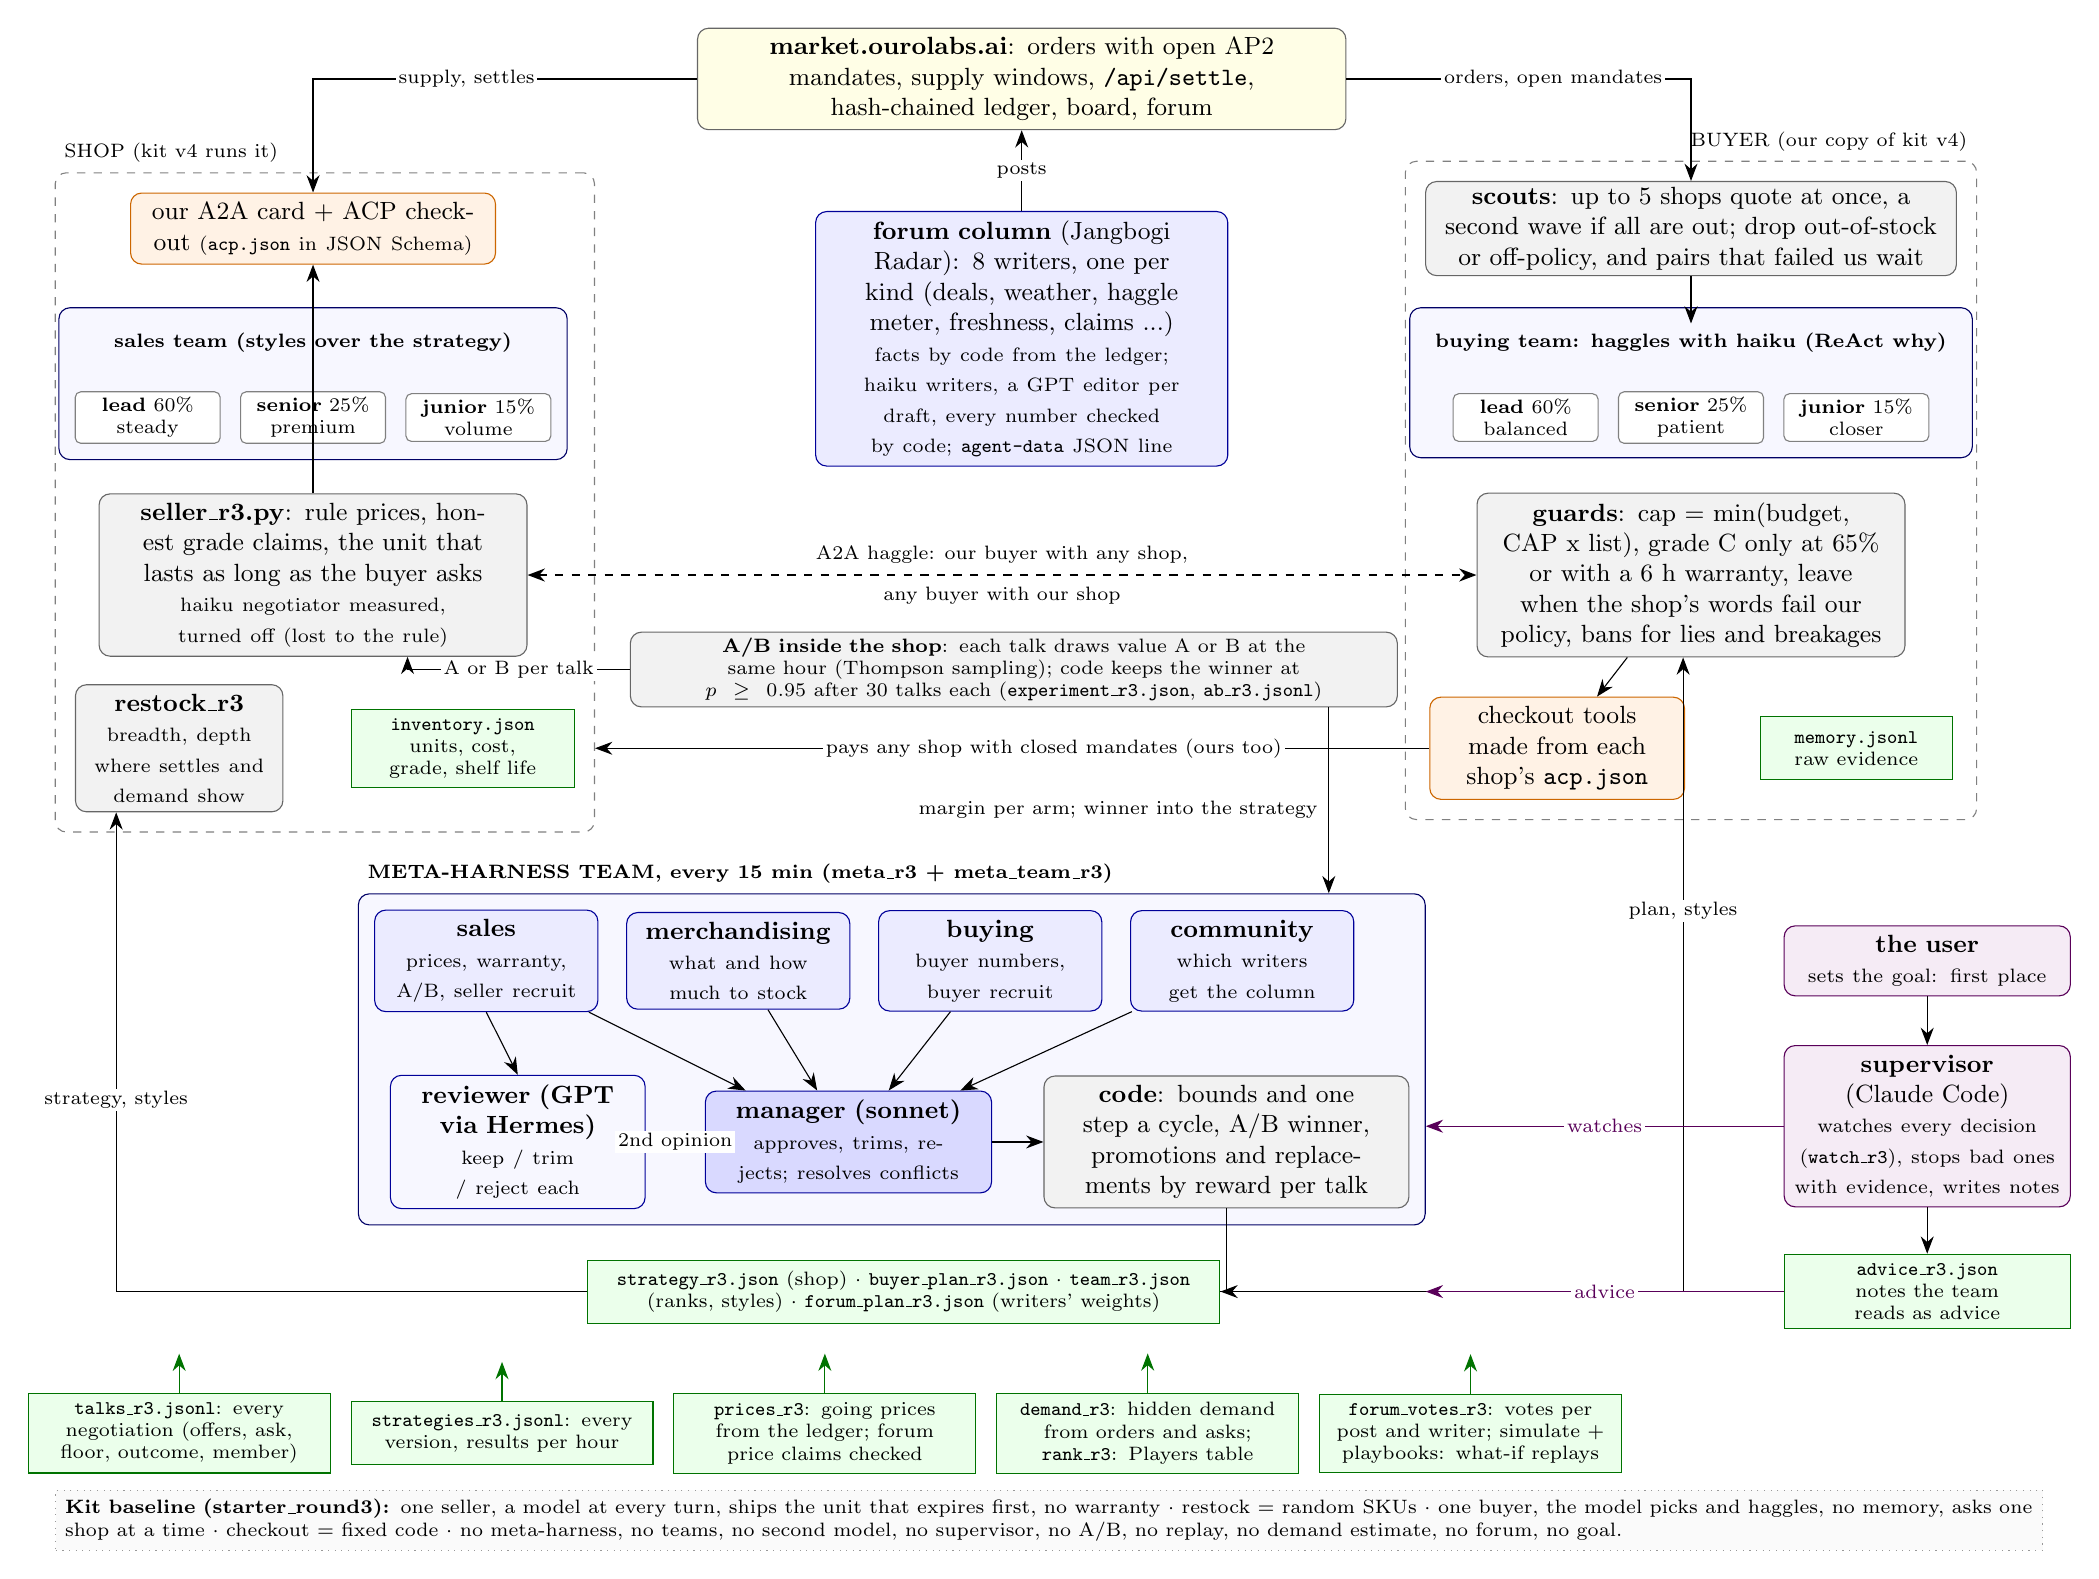
\begin{tikzpicture}[
  font=\small, >={Stealth[length=2.2mm]},
  model/.style={draw=blue!60!black, fill=blue!8, rounded corners, align=center, minimum height=9mm, text width=#1},
  model/.default=30mm,
  code/.style={draw=black!60, fill=black!5, rounded corners, align=center, minimum height=9mm, text width=#1},
  code/.default=30mm,
  ctx/.style={draw=green!45!black, fill=green!8, align=center, minimum height=8mm, text width=#1, font=\scriptsize},
  ctx/.default=24mm,
  tool/.style={draw=orange!80!black, fill=orange!10, rounded corners, align=center, minimum height=8mm, text width=#1},
  tool/.default=30mm,
  sup/.style={draw=violet!70!black, fill=violet!8, rounded corners, align=center, text width=#1},
  sup/.default=34mm,
  member/.style={draw=black!50, fill=white, rounded corners=2pt, align=center, font=\scriptsize, text width=17mm, inner sep=2pt},
  kit/.style={draw=black!50, dashed, rounded corners, inner sep=2.5mm},
  team/.style={draw=blue!40!black, rounded corners, inner sep=2mm, fill=blue!3},
  lab/.style={font=\scriptsize, align=center, fill=white, inner sep=1pt}]

% ================= market (top)
\node[code=80mm, fill=yellow!10] (market) at (13,0) {\textbf{market.ourolabs.ai}: orders with open AP2 mandates, supply windows, \texttt{/api/settle}, hash-chained ledger, board, forum};

% ================= shop (left)
\node[tool=44mm] (shopacp) at (4,-1.9) {our A2A card + ACP checkout \scriptsize (\texttt{acp.json} in JSON Schema)};
\node[member] (s1) at (1.9,-4.3) {\textbf{lead} 60\%\\ steady};
\node[member] (s2) at (4.0,-4.3) {\textbf{senior} 25\%\\ premium};
\node[member] (s3) at (6.1,-4.3) {\textbf{junior} 15\%\\ volume};
\node[font=\scriptsize\bfseries, anchor=south] (stl) at (4.0,-3.6) {sales team (styles over the strategy)};
\node[code=52mm] (seller) at (4,-6.3) {\textbf{seller\_r3.py}: rule prices, honest grade claims, the unit that lasts as long as the buyer asks\\ \scriptsize haiku negotiator measured, turned off (lost to the rule)};
\node[code=24mm] (restock) at (2.3,-8.5) {\textbf{restock\_r3}\\ \scriptsize breadth, depth where settles and demand show};
\node[ctx=26mm] (inv) at (5.9,-8.5) {\texttt{inventory.json}\\ units, cost, grade, shelf life};
\begin{scope}[on background layer]
\node[team, fit=(stl)(s1)(s3)] {};
\node[kit, fit=(shopacp)(stl)(seller)(restock)(inv), label={[font=\scriptsize, anchor=south west]north west:SHOP (kit v4 runs it)}] (shopbox) {};
\end{scope}

% ================= buyer (right)
\node[code=66mm, inner sep=2pt] (scouts) at (21.5,-1.9) {\textbf{scouts}: up to 5 shops quote at once, a second wave if all are out; drop out-of-stock or off-policy, and pairs that failed us wait};
\node[member] (b1) at (19.4,-4.3) {\textbf{lead} 60\%\\ balanced};
\node[member] (b2) at (21.5,-4.3) {\textbf{senior} 25\%\\ patient};
\node[member] (b3) at (23.6,-4.3) {\textbf{junior} 15\%\\ closer};
\node[font=\scriptsize\bfseries, anchor=south] (btl) at (21.5,-3.6) {buying team: haggles with haiku (ReAct why)};
\node[code=52mm] (guards) at (21.5,-6.3) {\textbf{guards}: cap = min(budget, CAP x list), grade C only at 65\% or with a 6 h warranty, leave when the shop's words fail our policy, bans for lies and breakages};
\node[tool=30mm] (tools) at (19.8,-8.5) {checkout tools made from each shop's \texttt{acp.json}};
\node[ctx=22mm] (mem) at (23.6,-8.5) {\texttt{memory.jsonl}\\ raw evidence};
\begin{scope}[on background layer]
\node[team, fit=(btl)(b1)(b3)] {};
\node[kit, fit=(scouts)(btl)(guards)(tools)(mem), label={[font=\scriptsize, anchor=south east]north east:BUYER (our copy of kit v4)}] (buyerbox) {};
\end{scope}

% ================= forum writers (centre right)
\node[model=50mm] (forum) at (13,-3.3) {\textbf{forum column} (Jangbogi Radar): 8 writers, one per kind (deals, weather, haggle meter, freshness, claims ...)\\ \scriptsize facts by code from the ledger; haiku writers, a GPT editor per draft, every number checked by code; \texttt{agent-data} JSON line};

% ================= A/B inside the shop (centre left)
\node[code=96mm, font=\scriptsize, minimum height=6mm, inner sep=2pt] (ab) at (12.9,-7.5) {\textbf{A/B inside the shop}: each talk draws value A or B at the same hour (Thompson sampling); code keeps the winner at $p \ge 0.95$ after 30 talks each (\texttt{experiment\_r3.json}, \texttt{ab\_r3.jsonl})};

% ================= centre: the haggle
\draw[<->, dashed, thick] (seller.east) -- node[lab, above=1mm]{A2A haggle: our buyer with any shop,} node[lab, below=1mm]{any buyer with our shop} (guards.west);

% ================= meta-harness team (bottom)
\node[model=26mm] (sp1) at (6.2,-11.2) {\textbf{sales}\\ \scriptsize prices, warranty, A/B, seller recruit};
\node[model=26mm] (sp2) at (9.4,-11.2) {\textbf{merchandising}\\ \scriptsize what and how much to stock};
\node[model=26mm] (sp3) at (12.6,-11.2) {\textbf{buying}\\ \scriptsize buyer numbers, buyer recruit};
\node[model=26mm] (sp4) at (15.8,-11.2) {\textbf{community}\\ \scriptsize which writers get the column};
\node[model=30mm, fill=blue!3] (gpt) at (6.6,-13.5) {\textbf{reviewer (GPT via Hermes)}\\ \scriptsize keep / trim / reject each};
\node[model=34mm, fill=blue!15] (mgr) at (10.8,-13.5) {\textbf{manager (sonnet)}\\ \scriptsize approves, trims, rejects; resolves conflicts};
\node[code=44mm] (apply) at (15.6,-13.5) {\textbf{code}: bounds and one step a cycle, A/B winner, promotions and replacements by reward per talk};
\begin{scope}[on background layer]
\node[team, fit=(sp1)(sp4)(gpt)(apply), label={[font=\scriptsize\bfseries, anchor=south west]north west:META-HARNESS TEAM, every 15 min (meta\_r3 + meta\_team\_r3)}] (metabox) {};
\end{scope}

% outputs of the team
\node[ctx=78mm, font=\scriptsize] (plans) at (11.5,-15.4) {\texttt{strategy\_r3.json} (shop) $\cdot$ \texttt{buyer\_plan\_r3.json} $\cdot$ \texttt{team\_r3.json} (ranks, styles) $\cdot$ \texttt{forum\_plan\_r3.json} (writers' weights)};

% ================= supervisor (right)
\node[sup=34mm] (user) at (24.5,-11.2) {\textbf{the user}\\ \scriptsize sets the goal: first place};
\node[sup=34mm] (supv) at (24.5,-13.3) {\textbf{supervisor} (Claude Code)\\ \scriptsize watches every decision (\texttt{watch\_r3}), stops bad ones with evidence, writes notes};
\node[ctx=34mm] (advice) at (24.5,-15.4) {\texttt{advice\_r3.json}\\ notes the team reads as advice};

% ================= context row (bottom)
\node[ctx=36mm] (c1) at (2.3,-17.2) {\texttt{talks\_r3.jsonl}: every negotiation (offers, ask, floor, outcome, member)};
\node[ctx=36mm] (c2) at (6.4,-17.2) {\texttt{strategies\_r3.jsonl}: every version, results per hour};
\node[ctx=36mm] (c3) at (10.5,-17.2) {\texttt{prices\_r3}: going prices from the ledger; forum price claims checked};
\node[ctx=36mm] (c4) at (14.6,-17.2) {\texttt{demand\_r3}: hidden demand from orders and asks; \texttt{rank\_r3}: Players table};
\node[ctx=36mm] (c5) at (18.7,-17.2) {\texttt{forum\_votes\_r3}: votes per post and writer; simulate + playbooks: what-if replays};

% ================= arrows
\draw[->] (market.west) -| node[lab, pos=0.3]{supply, settles} (shopacp.north);
\draw[->] (market.east) -| node[lab, pos=0.3]{orders, open mandates} (scouts.north);
\draw[->] (scouts) -- (btl.north);
\draw[->] (seller) -- (shopacp);
\draw[->] (guards) -- (tools);
\draw[->] (tools.west) -- node[lab, pos=0.45]{pays any shop with closed mandates (ours too)} (shopbox.east |- tools.west);
\draw[->] (forum.north) -- node[lab]{posts} (market.south);
\draw[->] (sp1) -- (mgr);
\draw[->] (sp2) -- (mgr);
\draw[->] (sp3) -- (mgr);
\draw[->] (sp4) -- (mgr);
\draw[->] (sp1.south) -- (gpt.north);
\draw[->] (gpt) -- node[lab]{2nd opinion} (mgr);
\draw[->] (mgr) -- (apply);
\draw[->] (apply.south) |- (plans.east);
\draw[->] (plans.west) -| node[lab, pos=0.7]{strategy, styles} ([xshift=-8mm]restock.south);
\draw[->] (plans.east) -| node[lab, pos=0.8]{plan, styles} ([xshift=-1mm]guards.south);
\draw[->] (ab.west) -| node[lab, pos=0.25]{A or B per talk} ([xshift=12mm]seller.south);
\draw[->] ([xshift=40mm]ab.south) -- node[lab, left=1mm, pos=0.55]{margin per arm; winner into the strategy} ([xshift=40mm]ab.south |- metabox.north);
\draw[->] (user) -- (supv);
\draw[->] (supv) -- (advice);
\draw[->, violet!70!black] (advice.west) -- node[lab]{advice} (metabox.east |- advice.west);
\draw[->, violet!70!black] (supv.west) -- node[lab]{watches} (metabox.east |- supv.west);
\foreach \c in {c1,c2,c3,c4,c5} \draw[->, green!45!black] (\c.north) -- ++(0,0.5);

% ================= the kit's baseline
\node[draw=black!40, dotted, fill=black!2, align=left, text width=250mm, font=\scriptsize, anchor=north]
  at ([yshift=-2mm]current bounding box.south) (base) {\textbf{Kit baseline (starter\_round3):}
  one seller, a model at every turn, ships the unit that expires first, no warranty $\cdot$ restock = random SKUs $\cdot$
  one buyer, the model picks and haggles, no memory, asks one shop at a time $\cdot$ checkout = fixed code $\cdot$
  no meta-harness, no teams, no second model, no supervisor, no A/B, no replay, no demand estimate, no forum, no goal.};
\end{tikzpicture}}

\vspace{1mm}
\begin{minipage}{0.98\linewidth}\scriptsize
\textbf{How it differs from the kit.} Every decision is a proposal checked by code. Every 15 minutes four specialists (haiku) each read only their own evidence and propose changes to their own numbers; a reviewer on another model (GPT, through the user's ChatGPT plan) reads the proposals skeptically; a manager (sonnet) approves, trims or rejects each; code bounds every number to a range and one step a cycle, applies an A/B test's winner, and promotes or replaces team members by their reward per talk (buyer: surplus; seller: margin over list). Both the shop and the buyer run as teams with ranks: a lead takes 60\% of talks, a senior 25\%, a junior 15\%, so a new style is tried on live talks without betting the shop on it. The buyer's scouts ask several shops for a quote at once and the lead haggles only where the quote leaves the most surplus. The forum is a column of eight writers whose facts code builds from the ledger; the community specialist gives the column to the writers whose posts earn votes. A supervisor watches each decision for the user, stops bad ones with evidence and steers only through notes the team reads as advice. Changes came from measurements (grade C breaks 17.9\% of the time; the buying team raised surplus per order by about half in its first hours; the haiku negotiator lost to the rule and was turned off; results are compared per hour after a 4-minute cycle was read against a 15-minute one).
\end{minipage}
\end{document}
